\documentclass[12pt]{article}

\usepackage{sbc-template}   % Template da SBC
\usepackage{graphicx,url}   % Suporte para figuras e URLs
\usepackage[brazil]{babel}  % Suporte ao português brasileiro
\usepackage[utf8]{inputenc} % Suporte a caracteres UTF-8
\usepackage{cite}           % Estilo numérico para citações
\usepackage{amsmath}        % Suporte a fórmulas matemáticas

\bibliographystyle{sbc}     % Estilo das referências no padrão SBC
\sloppy                     % Corrige problemas de justificação

\title{Algoritmo Guloso vs. Backtracking: Coloração de Vértices em Grafos}

\author{
    Alef Cauan Sousa Rodrigues -- Matrícula: 20239000304\inst{1} \\
    Daniel Rodrigues de Sousa -- Matrícula: 20239006489\inst{1} \\
    Rayssa dos Santos Alves -- Matrícula: 20239019558\inst{1} \\
}

\address{Universidade Federal do Piauí - Campus Senador Helvídio Nunes Barros (UFPI)\\
  Caixa Postal 64049-55 -- 64.600-000 -- Picos -- PI -- Brasil
}

\begin{document}

\maketitle

\section{Introdução}
O problema de coloração de vértices é um dos problemas NP-completos mais estudados em grafos, com vastas aplicações em diversas áreas. — Diestel, R. (2017). Graph Theory (5th ed.). Springer. (Você pode encontrar informações sobre o livro e, às vezes, acesso a capítulos em SpringerLink). A coloração de vértices em grafos é um problema clássico na teoria dos grafos, onde o objetivo é atribuir cores aos vértices de um grafo, de maneira que nenhum par de vértice adjacente, conectado por uma aresta, tenha a mesma cor. Este problema possui diversas aplicações práticas em áreas como o planejamento de horários, a alocação de frequências. A complexidade e a busca pela solução ótima para a coloração de grafos tornam-na um campo de estudo relevante, impulsionando a comparação entre diferentes abordagens algoritmicas, como o Guloso e o Backtracking. 

O Algoritmo guloso é uma classe de algoritmos que faz a escolha que parece a melhor no momento presente  — Cormen, T. H., Leiserson, C. E., Rivest, R. L.,  Stein, C. (2009). Introduction to Algorithms (3rd ed.). MIT Press. O algoritmo guloso é uma estratégia de otimização que toma decisões ótimas localmente em cada etapa, com a esperança de que essas escolhas levem a uma solução globalmente ótima. No contexto da coloração de grafos, isso geralmente significa atribuir a menor cor disponível a um vértice, sem considerar as implicações futuras dessa decisão. Mesmo que essa técnica seja eficiente em termos de execução e simplicidade, mas a solução encontrada pode não ser a melhor solução do problema, levando a uma solução subótima.

Backtracking é uma técnica algorítmica para resolver problemas recursivamente, especialmente aqueles que buscam encontrar todas as soluções ou uma solução ótima, construindo candidatas a soluções uma a uma e removendo aquelas que falham em satisfazer as restrições do problema. —- Knuth, D. E. (1997). The Art of Computer Programming, Volume 1: Fundamental Algorithms (3rd ed.). O algoritmo backtracking adota abosrdagens mais sistemáticas e exaustivas, ela explora todas as possíveis atribuições de cores para a construção de uma solução ótima, retrocedendo o passo para o anterior, caso a sub solução não puder ser estendida para uma solução completa válida. Embora essa solução seja computacionalmente mais custosa, ela encontrará a melhor solução para o problema, mesmo que seja preciso entrar em todos os casos possíveis.


\section{Metodologia}

Para avaliar as duas abordagens, foram implementados algoritmos em Python e testados com grafos de tamanhos variados (10, 15, 20, 25 e 50 vértices), mantendo uma densidade de arestas fixa em 0.4.

\subsection{Algoritmo Guloso}

O algoritmo guloso implementado utiliza uma abordagem direta para colorir os vértices do grafo, processando cada vértice sequencialmente e atribuindo a primeira cor disponível que não cause conflitos com os vértices adjacentes.

\begin{itemize}
    \item \textbf{Entrada}: Um grafo \( G \) representado por uma lista de adjacência e um conjunto de cores disponíveis.
    \item \textbf{Processo}:
    \begin{enumerate}
        \item Inicializa um array de cores com tamanho igual ao número de vértices.
        \item Para cada vértice \( v \) do grafo:
        \begin{itemize}
            \item Coleta o conjunto de cores já utilizadas pelos vértices adjacentes.
            \item Atribui a primeira cor disponível que não está no conjunto de cores utilizadas.
        \end{itemize}
    \end{enumerate}
    \item \textbf{Complexidade}: O algoritmo tem complexidade temporal de \( O(V + E) \), onde \( V \) é o número de vértices e \( E \) o número de arestas.
\end{itemize}

A implementação inclui otimizações importantes:
\begin{itemize}
    \item Utiliza um conjunto (set) para rastrear cores utilizadas, permitindo verificação em \( O(1) \).
    \item Processa os vértices em ordem natural, reduzindo overhead de ordenação.
    \item Mantém uma lista fixa de cores pré-definidas para consistência nos resultados.
\end{itemize}

Para garantir a validade dos experimentos, o algoritmo:
\begin{itemize}
    \item Opera sobre grafos conexos gerados aleatoriamente com densidade controlada (0.4).
    \item Mantém os pesos das arestas entre 1 e 15 para simular situações reais.
    \item Inclui métricas de tempo e memória usando \texttt{time.perf\_counter()} e \texttt{tracemalloc}.
\end{itemize}

\subsection{Algoritmo de Backtracking}

O algoritmo de backtracking adota uma abordagem mais completa, explorando todas as possibilidades de coloração de forma sistemática. Ele tenta todas as combinações possíveis até encontrar uma coloração válida, retrocedendo (backtrack) sempre que encontra um impasse.

\begin{itemize}
    \item \textbf{Entrada}: Um grafo \( G \) e um número máximo de cores \( k \).
    \item \textbf{Processo}:
    \begin{enumerate}
        \item Para cada vértice:
        \begin{itemize}
            \item Tenta atribuir uma cor de 1 a \( k \).
            \item Verifica se a cor é válida (nenhum vizinho tem a mesma cor).
            \item Se for válida:
            \begin{itemize}
                \item Avança para o próximo vértice de forma recursiva.
                \item Se a tentativa falhar, desfaz a escolha e tenta a próxima cor.
            \end{itemize}
        \end{itemize}
    \end{enumerate}
    \item \textbf{Complexidade}: A complexidade é \( O(k^V) \), devido à explosão combinatória de possibilidades.
\end{itemize}

Apesar de ser mais custoso computacionalmente, o backtracking garante encontrar uma solução, se ela existir, e pode utilizar um número mínimo de cores em certos casos.

\subsection{Critérios de Avaliação}

A análise comparativa entre os algoritmos considera os seguintes aspectos:

\begin{itemize}
    \item Tempo de execução para diferentes tamanhos de grafos.
    \item Uso de memória durante a execução.
    \item Número de cores utilizadas na coloração final.
\end{itemize}

\section{Resultados}
Nesta secção serão apresentados os resultados dos testes realizados com comparativos entre as duas implementações do guloso e a do backtracking.
\subsection{Comparação de Uso de Memória}

O gráfico da Figura \ref{fig:mem} apresenta uma comparação do uso de memória (em KB) dos algoritmos Backtracking Puro, Guloso em Ordem e Guloso por Grau, para grafos com 10, 15, 20, 25 e 50 vértices. Observa-se que o Backtracking Puro (barras azuis) exibe um consumo de memória significativamente maior, especialmente para grafos maiores. Para 10 vértices, o uso é de aproximadamente 20 KB, mas aumenta drasticamente para cerca de 140 KB com 50 vértices, refletindo a natureza recursiva e exaustiva do algoritmo, que armazena múltiplos estados durante a busca pela solução ótima.

\begin{figure}[!htb]
    \centering
    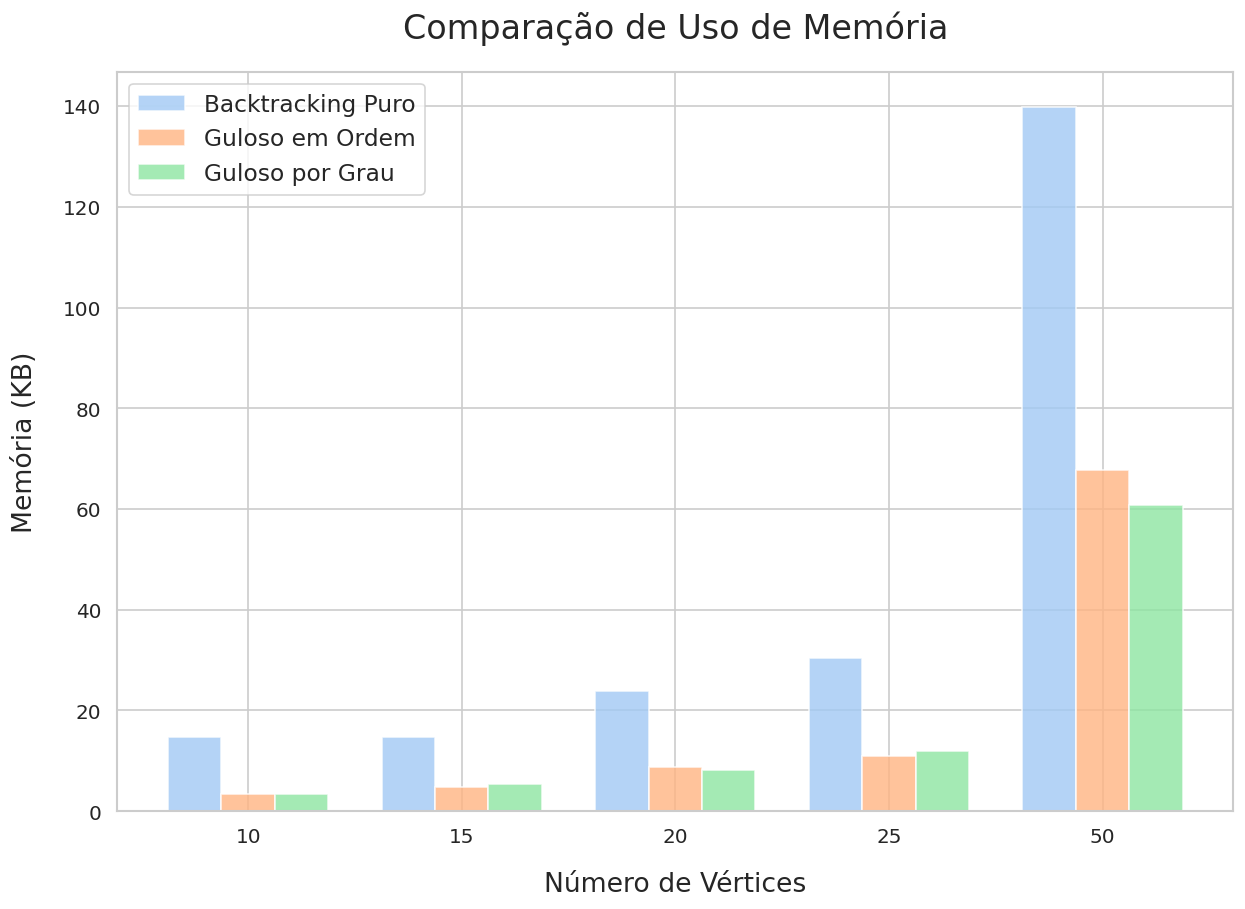
\includegraphics[width=0.5\linewidth]{imgs/comparativo_memoria.png}
    \caption{Uso de memória}
    \label{fig:mem}
\end{figure}


Por outro lado, os algoritmos gulosos apresentam um uso de memória muito mais eficiente. O Guloso em Ordem (barras laranjas) consome cerca de 5 KB para 10 vértices, crescendo para 60 KB com 50 vértices, enquanto o Guloso por Grau (barras verdes) consome 6 KB para 10 vértices e 70 KB para 50 vértices. A diferença entre os dois algoritmos gulosos é pequena, mas o Guloso por Grau utiliza um pouco mais de memória devido ao cálculo e ordenação dos graus dos vértices. Ambos os algoritmos gulosos mostram um crescimento mais linear no uso de memória, tornando-os mais adequados para grafos maiores em comparação com o Backtracking Puro.

\subsection{Comparação de Tempo de Execução}

A Figura \ref{fig:temp} ilustra a comparação do tempo de execução (em milissegundos) dos algoritmos Backtracking Puro, Guloso em Ordem e Guloso por Grau, para grafos com número de vértices variando de 10 a 50. O Backtracking Puro (linha azul com círculos) apresenta um crescimento exponencial no tempo de execução, começando próximo de 0 ms para 10 vértices, mas atingindo cerca de 15 ms para 50 vértices. Esse comportamento reflete a complexidade exponencial do algoritmo, que testa todas as combinações possíveis de cores para encontrar a solução ótima, tornando-o impraticável para grafos maiores.

\begin{figure}[!htb]
    \centering
    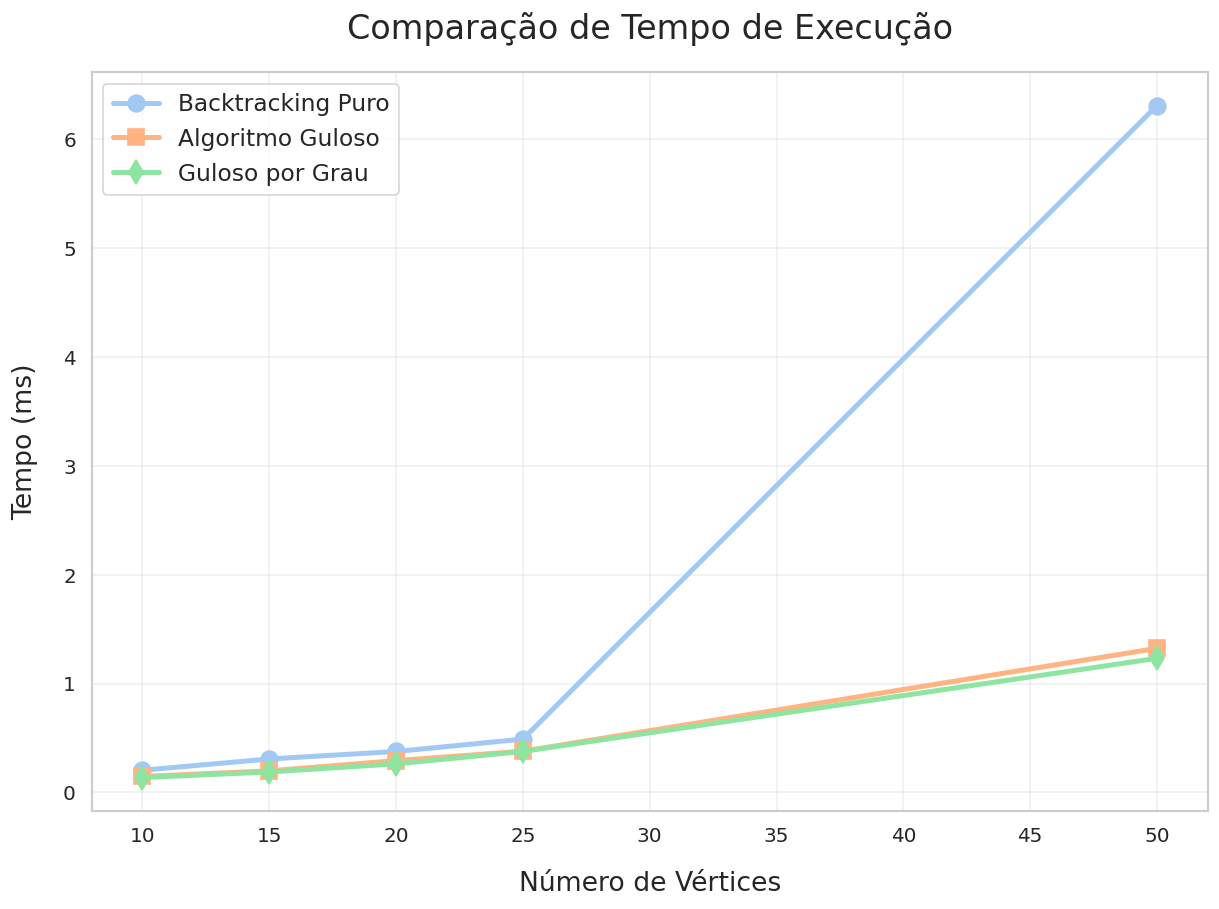
\includegraphics[width=0.6\linewidth]{imgs/comparativo_tempo.png}
    \caption{Uso de Tempo}
    \label{fig:temp}
\end{figure}


Em contraste, os algoritmos gulosos demonstram um desempenho muito superior. O Guloso em Ordem (linha laranja com quadrados) mantém tempos de execução extremamente baixos, crescendo de 0 ms para 10 vértices até aproximadamente 1 ms para 50 vértices. O Guloso por Grau (linha verde com triângulos) segue um padrão semelhante, mas é ligeiramente mais lento, alcançando cerca de 1,2 ms para 50 vértices, devido ao custo adicional de ordenar os vértices por grau (\( O(V \log V) \)). Ambos os algoritmos gulosos exibem um crescimento quase linear no tempo de execução, destacando sua eficiência e escalabilidade em comparação com o Backtracking Puro.

\section{Conclusão}

Este estudo comparativo entre os algoritmos Guloso e Backtracking para coloração de vértices em grafos revelou importantes trade-offs entre eficiência computacional e qualidade da solução. Os resultados experimentais demonstram que:

\begin{itemize}
    \item O algoritmo Guloso apresenta desempenho superior em termos de tempo de execução e uso de memória, com crescimento quase linear em relação ao tamanho do grafo, tornando-o mais adequado para aplicações práticas com grafos grandes.
    
    \item O Backtracking, embora garanta encontrar a solução ótima quando existe, apresenta crescimento exponencial tanto em tempo quanto em memória, limitando sua aplicabilidade a grafos menores.
    
    \item A diferença de performance se torna mais expressiva conforme o tamanho do grafo aumenta, com o Backtracking consumindo até 140 KB de memória para 50 vértices, enquanto o Guloso mantém um uso mais modesto de 60-70 KB.
\end{itemize}

Na prática, a escolha entre os dois algoritmos dependerá das necessidades específicas da aplicação. Para cenários onde a eficiência é prioritária e soluções aproximadas são aceitáveis, o algoritmo Guloso é claramente a melhor opção. Por outro lado, em situações onde a otimalidade da solução é crucial e o tamanho do grafo é limitado, o Backtracking pode ser mais apropriado.

\vspace{1cm}

\bibliography{referencias}  
\end{document}
